\documentclass{standalone}

\usepackage{tikz}
\usetikzlibrary{fit,positioning,calc}

\usepackage{pgfplots}
\pgfplotsset{
    compat=1.16,
}
\usepgfplotslibrary{external}
\tikzexternalize[
    only named,
]

\definecolor{pblue}{RGB}{0,102,189}  % precice blue
\definecolor{porange}{RGB}{243,98,33}  % precice orange

% Make the 'export as png' a seperate style, with default density 200
\tikzset{
    export as png/.style={
        external/system call/.add={}{
            && convert -density #1 -transparent white "\image.pdf" "\image.png"
        },
    },
    export as png/.default={200},
}

\begin{document}

\tikzset{export as png}
\tikzsetnextfilename{tutorials-partitioned-heat-conduction-schwarz-setup}
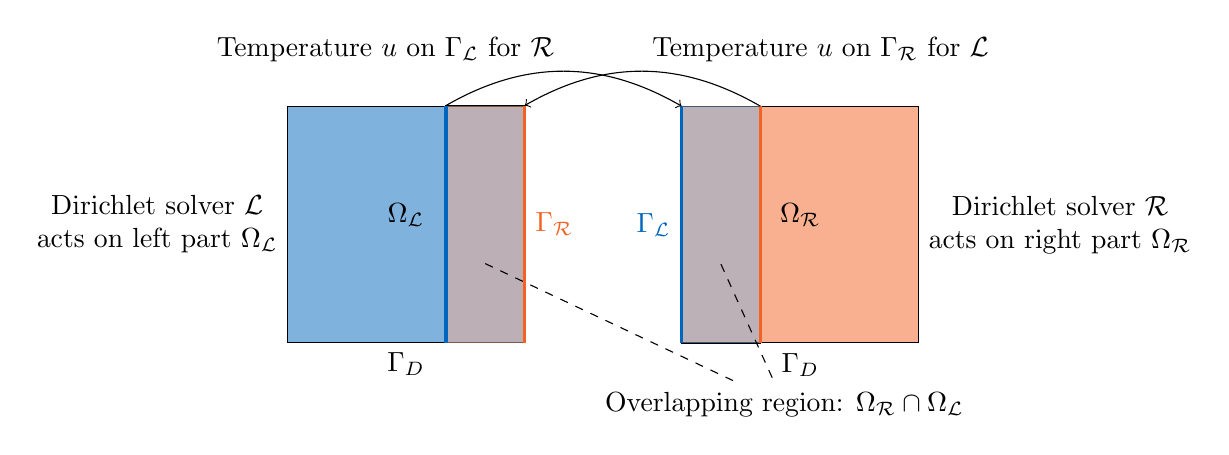
\begin{tikzpicture}
    \draw
        (0,0) coordinate (a)
        rectangle
        ++(3,3) coordinate (b);
    \node[fill=pblue!50, draw=black, fit=(a) (b),inner sep=0pt] (participantL) {$\Omega_\mathcal{L}$};

    \draw
        ($(participantL.south east)+(2,0)$) coordinate (a)
        rectangle
        ++(3,3) coordinate (b);
    \node[fill=porange!50, draw=black, fit=(a) (b),inner sep=0pt] (participantR) {$\Omega_\mathcal{R}$};

    \draw
        ($(participantL.south east)-(1,0)$) coordinate (a)
        rectangle
        ($(participantL.north east)$) coordinate (b);
    \node[fill=porange!50,opacity=0.5, fit=(a) (b),inner sep=0pt] (overlapL){};

    \draw
        ($(participantR.south west)+(1,0)$) coordinate (a)
        rectangle
        ($(participantR.north west)$) coordinate (b);
    \node[fill=pblue!50,opacity=0.5, fit=(a) (b),inner sep=0pt] (overlapR){};

    \node[below = 0.5cm of participantR,xshift=-0.2cm](overlapLabel){Overlapping region: $\Omega_\mathcal{R}\cap\Omega_\mathcal{L}$};
    \draw[dashed] ([yshift=-.5cm]overlapL.center) -- (overlapLabel);
    \draw[dashed] ([yshift=-.5cm]overlapR.center) -- (overlapLabel);

    \draw[very thick, pblue]($(participantL.south east)-(1,0)$) -- ($(participantL.north east)-(1,0)$);
    \draw[very thick, porange]($(participantR.south west)+(1,0)$) -- ($(participantR.north west)+(1,0)$);

    \draw[very thick, porange](participantL.south east) -- node[right]{$\Gamma_\mathcal{R}$}($(participantL.north east)$);
    \draw[very thick, pblue](participantR.south west) -- node[left]{$\Gamma_\mathcal{L}$} ($(participantR.north west)$);

    \node[left = 0cm of participantL,align=center] {Dirichlet solver $\mathcal{L}$\\ acts on left part $\Omega_\mathcal{L}$};
    \node[right = 0cm of participantR,align=center] {Dirichlet solver $\mathcal{R}$\\ acts on right part $\Omega_\mathcal{R}$};

    \draw[->]($(participantR.north west)+(1,0)$) to[out=150,in=30] node[above right,align=center]{Temperature $u$ on $\Gamma_\mathcal{R}$ for $\mathcal{L}$} (participantL.north east);
    \draw[->]($(participantL.north east)-(1,0)$) to[out=30,in=150] node[above left,align=center]{Temperature $u$ on $\Gamma_\mathcal{L}$ for $\mathcal{R}$} (participantR.north west);

    \draw[draw=none] (participantL.south east) -- node[below]{$\Gamma_D$} (participantL.south west);
    \draw[draw=none] (participantR.south east) -- node[below]{$\Gamma_D$} (participantR.south west);
\end{tikzpicture}

\end{document}